%Template v.1.0: Taylor Arnold and Simon Gabay, december 2025
% CECI EST UN FICHIER DE MODÈLE LATEX POUR LES ARTICLES INCLUS DANS
% *Anthology of Computers and the Humanities*. AJOUTEZ L'OPTION
% 'final' LORS DE LA CRÉATION DE LA VERSION FINALE DE L'ARTICLE. 
% NE PAS modifier la classe du document
%\documentclass[final, fra, custom]{anthology-ch}     
% pour la version finale
\documentclass[final, fra]{anthology-ch}      
% pour la soumission

% CHARGER LES PACKAGES LaTeX
\usepackage{booktabs}
\usepackage{graphicx}
\usepackage{subcaption}
\usepackage{todonotes}

% AJOUTEZ vos propres packages avec \usepackage{}

% TITRE DE LA SOUMISSION
% Remplacez ceci par le titre de votre soumission
\title{Marot, Malingre ou Beaulieu? Sur l'attribution de la \textit{Chanson spirituelle} (1545)}

% INFORMATIONS SUR LES AUTEURS ET LES AFFILIATIONS
% Pour chaque auteur, utilisez une nouvelle commande \author, avec
% les numéros entre crochets indiquant les affiliations correspondantes
% (section suivante) et l'ORCID-ID pour chaque auteur.  
\author[1]{Sonia Solfrini}[
  orcid=0009-0009-7367-048X,
  email=sonia.solfrini@unige.ch
]
\author[1]{Simon Gabay}[
  orcid=0000-0001-9094-4475
]

% SS : comment transformer "and" en "et ??

% Il doit y avoir un appel à \affiliation pour chaque affiliation des auteurs.
% Plusieurs affiliations peuvent être attribuées à un auteur
% et une affiliation peut être attribuée à plusieurs auteurs. 
\affiliation{1}{Université de Genève, Suisse}

% MOTS-CLÉS
% Fournissez un ou plusieurs mots-clés séparés par des virgules
% en utilisant les commandes suivantes
\keywords[fra]{stylométrie, attribution d'auteur, philologie computationnelle, Renaissance}
\keywords[eng]{stylometry, authorship attribution, computational philology, renaissance}

% MÉTADONNÉES DE LA PUBLICATION
% Ces champs seront remplis lors de la publication ; 
% ils peuvent être laissés par défaut lors de la soumission
\pubyear{2026}
\pubvolume{4}
\pagestart{44}
\pageend{54}
\paperorder{6}
\conferencename{Actes de la Conférence Humanistica}
\conferenceeditors{Serena Crespi, Simon Gabay, Martin Grandjean, Ariane Pinche, Marie Puren et Léa Saint-Raymond}
\doi{10.63744/DP4G7d5uBMeW}
\customhead{}

\addbibresource{bibliography.bib}

%%%%%%%%%%%%%%%%%%%%%%%%%%%%%%%%%%%%%%%%%%%%%%%%%%%%%%%%%%%%%%%%%%%%%%%%%%%

% DÉBUT DU TEXTE
\begin{document}

\maketitle

\begin{abstract}
%Ce modèle LaTeX vous aide à composer et formater un article dans l'Anthologie d'ACH. En pratique, le résumé de l'article doit être un paragraphe rédigé en anglais synthétisant le plan et les principales contributions de l'article. 
This paper investigates the authorship of the \textit{Chanson spirituelle} (1545), an anonymous collection whose attribution has been variously linked to the poets Clément Marot, Eustorg de Beaulieu, and especially Matthieu Malingre. Using a stylometric approach, selected anonymous verses from the collection are compared against balanced corpora of approximately $6~000$ words for each of the three candidate authors. Although the results must be interpreted cautiously, given the absence of any clear positive signal, they suggest that the different pieces of the collection may not have been written by the same author.
\end{abstract}

\section{Introduction}
\label{sec:intro}

Matthieu Malingre (ca.~1500-1572) est un poète français du \textsc{xvi}\textsuperscript{e} siècle, proche des cercles évangéliques réfugiés dans l'espace suisse romand \cite{solfaroli2024pratiche, szczech2019ravir, gross2018theatre, ferrer2012chanson}. Le seul texte où son nom apparaît sur une page de titre est \textit{L'Epistre de M. Malingre envoyée a Clement Marot}, publiée par Jacques Estauge à Bâle en 1546. Tous les autres écrits attribués à Malingre sont publiés sous couvert d'anonymat ou par le biais de signatures obliques qui recourent à des jeux de mots. C'est le cas pour le nom de plume «~Gramelin~» et la devise «~Y me vint mal à gré~», qui contiennent des anagrammes de Malingre. Dans d'autres cas, son identité est dissimulée dans des acrostiches 
(fig.~\ref{fig:exemples_malingre}) 
\cite{gross2007acrostiches,bodenmann_lauteur_2009}. 

C'est grâce à ce type de signatures que quatre publications imprimées entre 1533 et 1535 par Pierre de Vingle sont attribuées à Malingre: une moralité, la \textit{Moralité de la maladie de Chrestienté} (1533), deux recueils de chansons spirituelles, les \textit{Noelz nouveaulx} (ca. 1533) et \textit{Plusieurs belles et bonnes chansons} (1533); ainsi que l'index des matières de la Bible d'Olivétan (1535). À ces imprimés publiés à Neuchâtel, nous ajoutons un poème manuscrit dont l'attribution à Malingre est étayée par la présence de deux acrostiches de son nom et de sa devise\footnote{Une étude de ce manuscrit inédit est actuellement en cours (S. S.).}.

D'autres textes, bien que parfois attribués à Malingre, ne comportent pas ses signatures obliques, ce qui rend leur attribution plus incertaine. Parmi ces œuvres figurent les \textit{Chansons nouvelles} (ca.~1534) et \textit{La Verité cachée} (ca.~1533), imprimées par Pierre de Vingle, ainsi que la \textit{Chanson spirituelle sur la saincte Cene} (1545), dont l'imprimeur et le lieu de publication demeurent inconnus. La critique s'accorde pour voir en Malingre l'auteur des \textit{Chansons nouvelles} (ca.~1534), mais la paternité des deux autres textes reste débattue.
Si la critique ne s'est jamais prononcée sur d'autres candidats possibles pour \textit{La Verité cachée}, les noms des poètes Clément Marot (1496-1544) \cite{berthon2014intention, berthon2019marot_bibliographie} et Eustorg de Beaulieu (ca.~1495-1552) \cite{goeury2018chrestienne,harvitt_eustorg_1918} ont en revanche été avancés pour la \textit{Chanson spirituelle} (cf. § \ref{sec:debat-cs}).

Afin de jeter un éclairage nouveau sur l'attribution de la \textit{Chanson spirituelle}, nous nous proposons d'utiliser une approche stylométrique.
Pour ce faire, nous confronterons certains pièces en vers de ce recueil à un corpus de textes en vers attribués à Malingre, Marot et Beaulieu.

\begin{figure*}
    \centering
    \medskip
    \begin{subfigure}[t]{.31\linewidth}
        \centering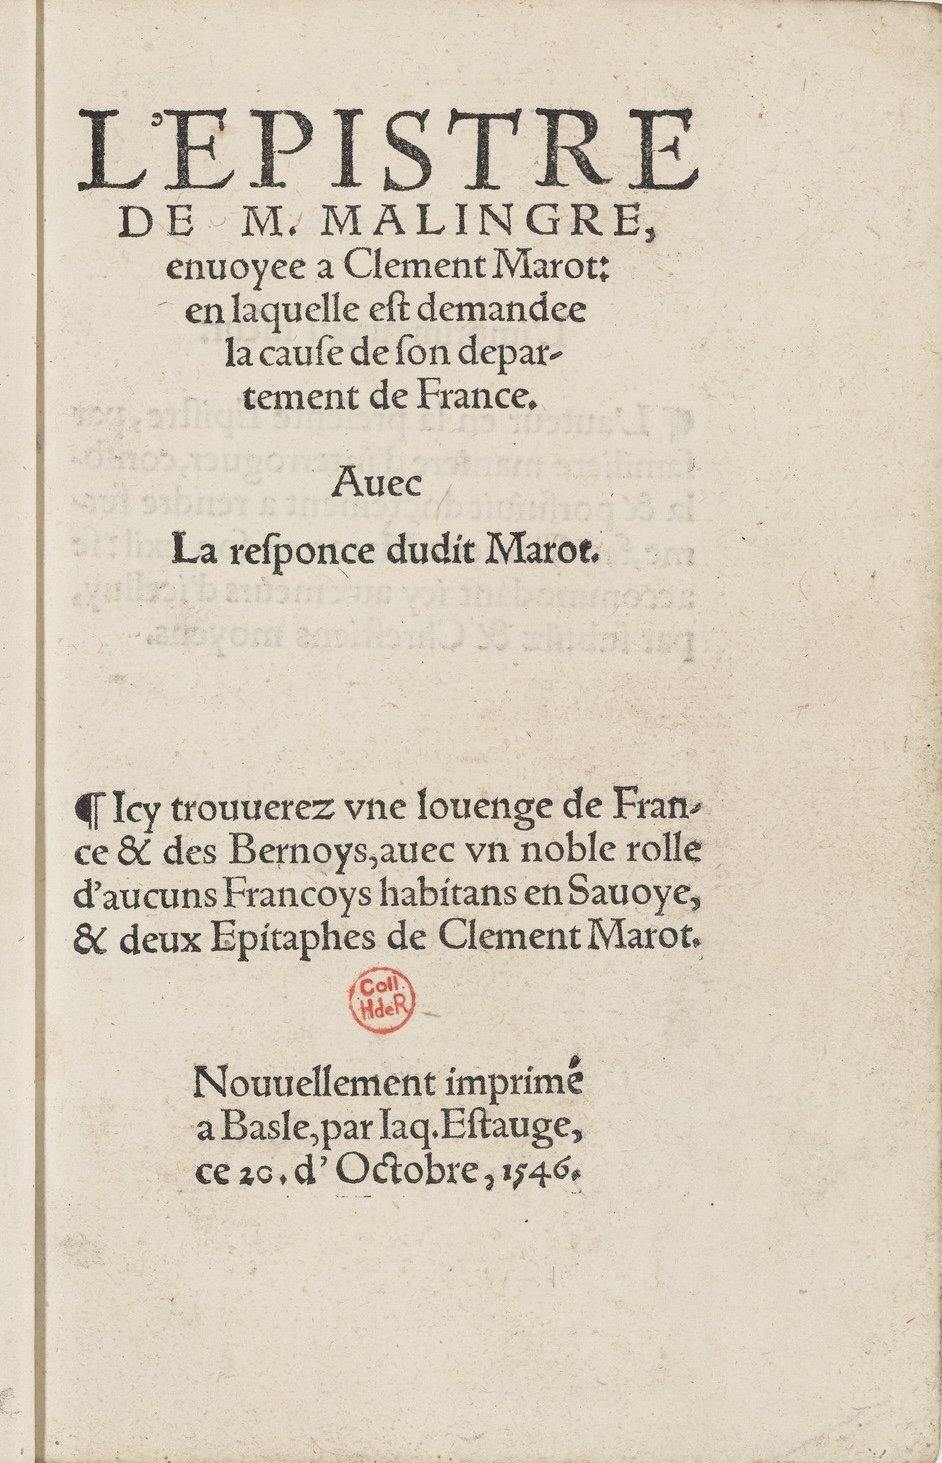
\includegraphics[width=.87\linewidth,height=6cm,keepaspectratio=false]{images/epistre-malingre-btv1b52524192b_9.jpeg}
        \caption{}
    \end{subfigure}
    \vspace{0.2cm}
    \hspace{0.2cm}%
    \begin{subfigure}[t]{.31\linewidth}
        \centering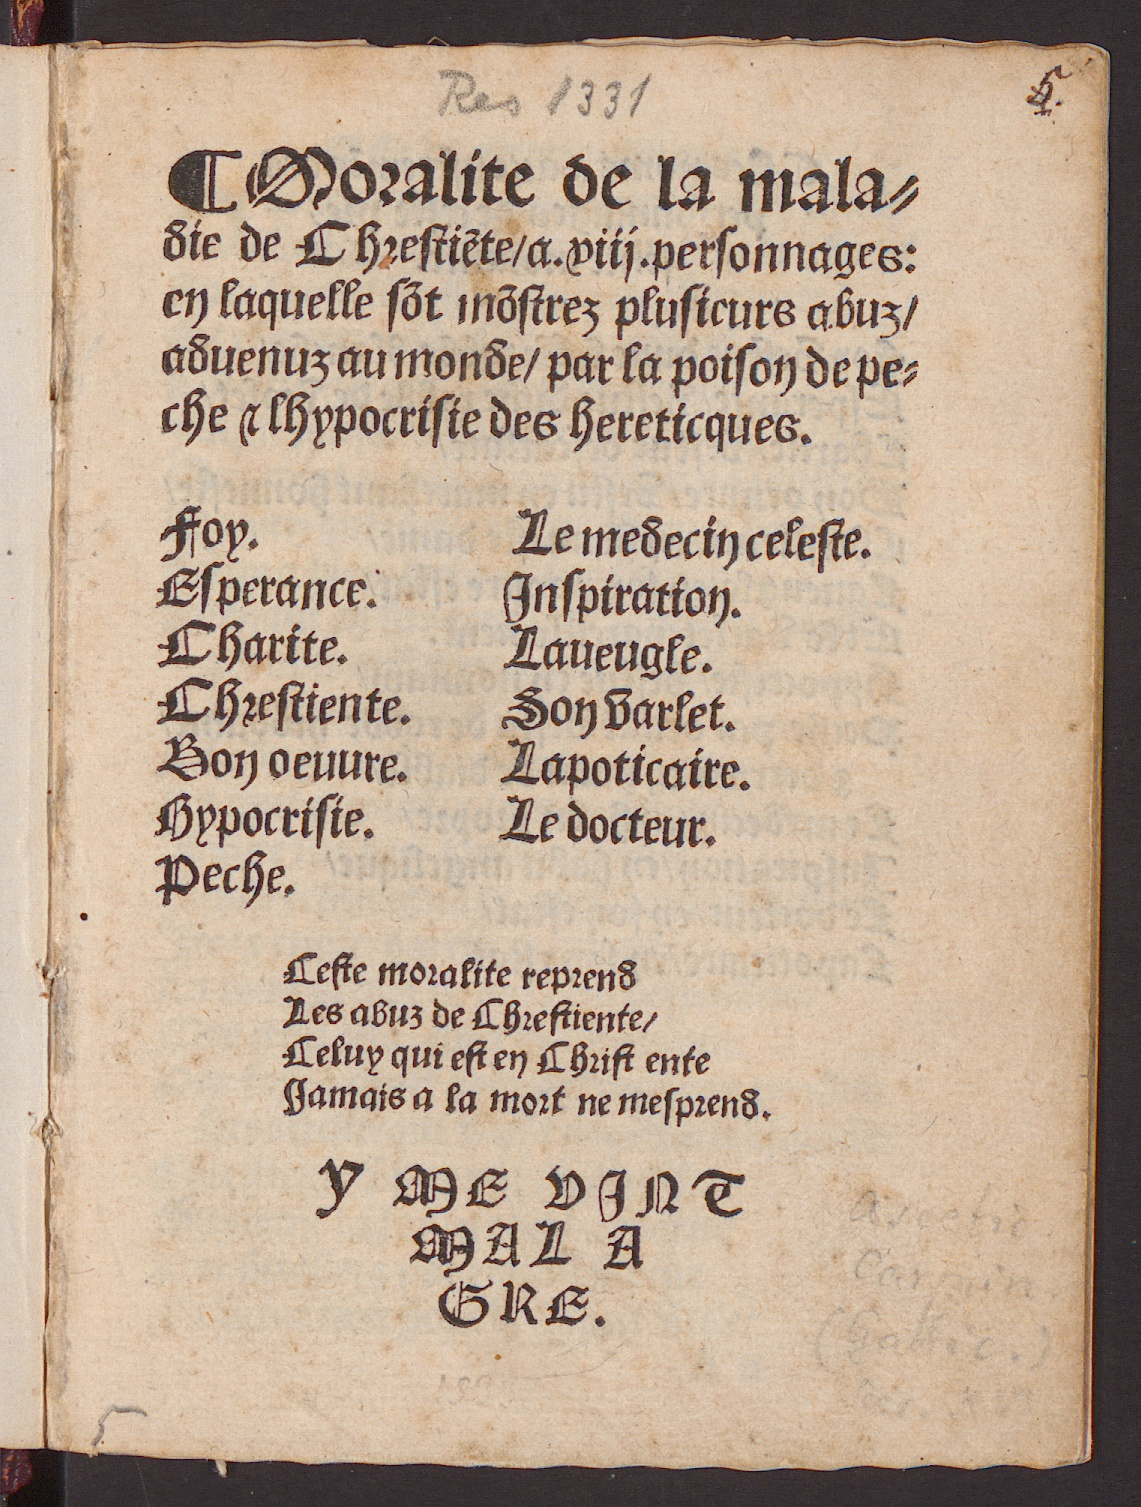
\includegraphics[width=.87\linewidth,height=6cm,keepaspectratio=false]{images/moralite-vingle-165304-original.jpg}
        \caption{}
    \end{subfigure}
    \vspace{0.2cm}
    \hspace{0.2cm}%
    \begin{subfigure}[t]{.31\linewidth}
        \centering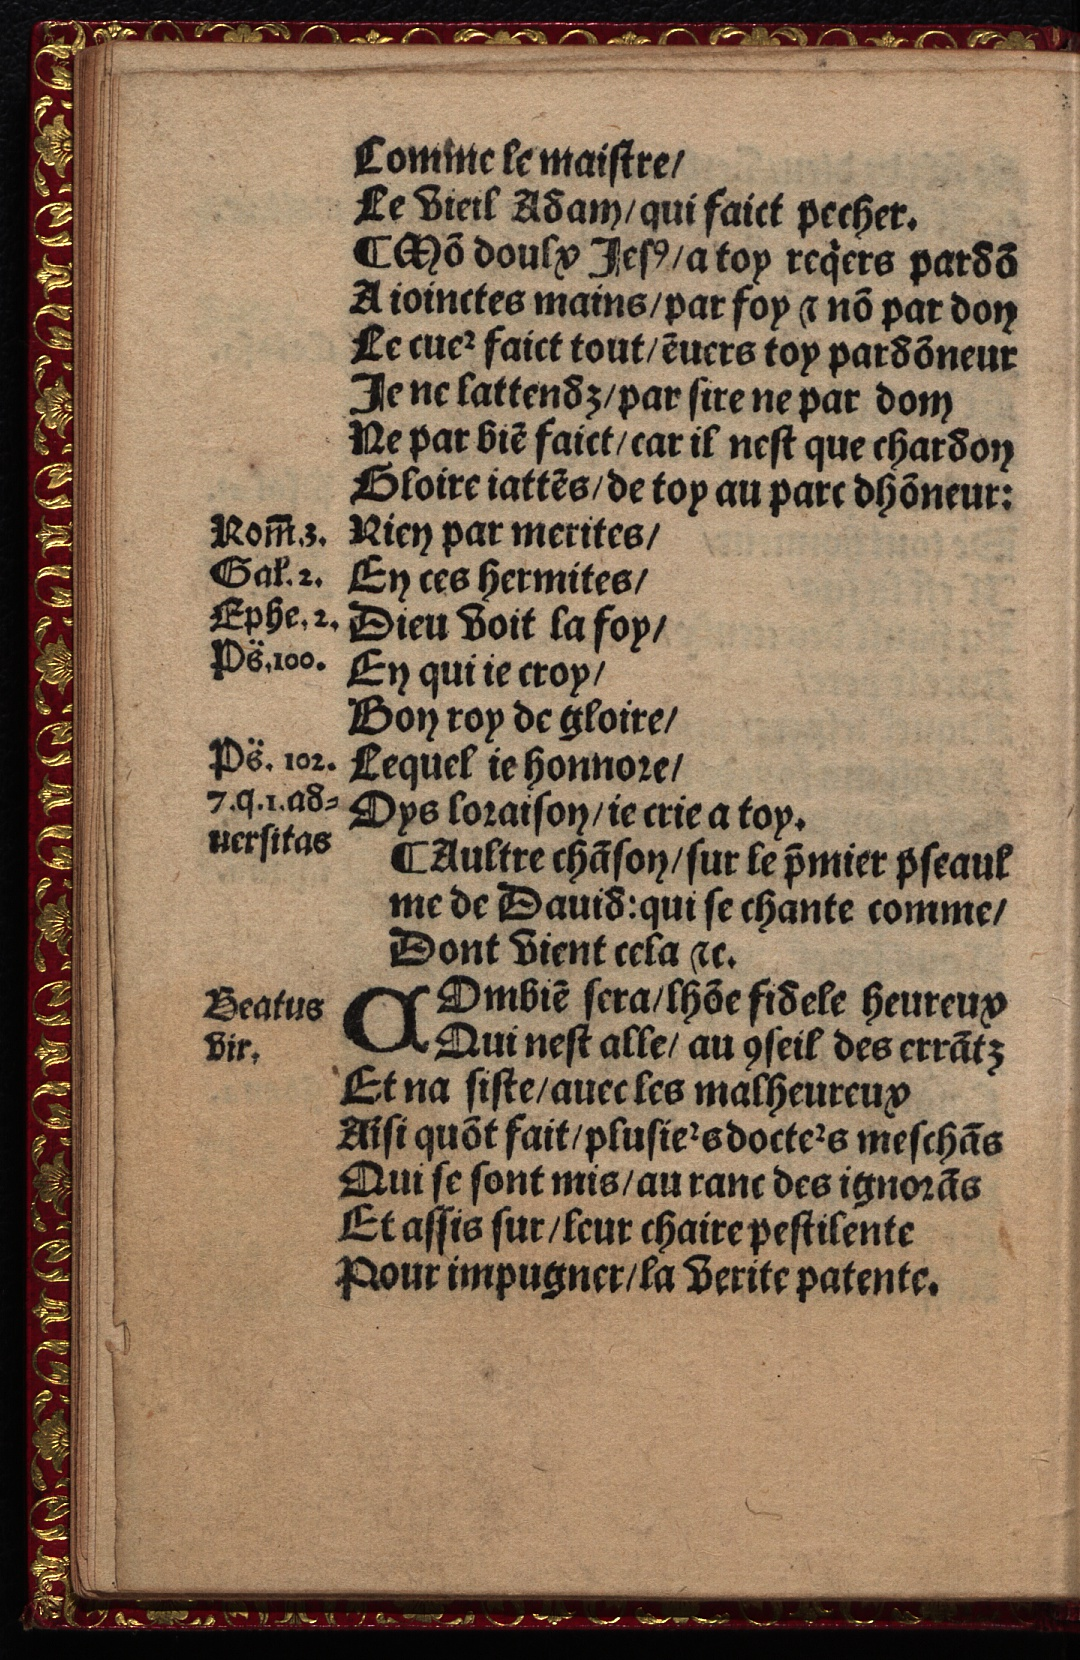
\includegraphics[width=.87\linewidth,height=6cm,keepaspectratio=false]{images/acrostiche-2031650-original.jpeg}
        \caption{}
    \end{subfigure}
    \vspace{-0.4cm}
  \caption{\textbf{(a)} Le nom de Malingre sur une page de titre. Source : \textit{L'Epistre de M. Malingre envoyée a Clement Marot}. Bâle : J. Estauge, 1546. (\href{https://gallica.bnf.fr/ark:/12148/btv1b52524192b}{\underline{Gallica}}) ; \textbf{(b)} La devise de Malingre, «~Y me vint mal à gré~», sur une page de titre. Source : \textit{Moralité de la maladie de Chrestienté}. [Neuchâtel]: [P. de Vingle], 1533. (\href{https://doi.org/10.3931/e-rara-563}{\underline{e-rara}}) ; \textbf{(c)} Un acrostiche de Malingre, «~Malingre de Bloys~», dans une chanson. Source : \textit{Plusieurs belles et bonnes chansons}. [Neuchâtel] : [P. de Vingle], 1533. (\href{https://doi.org/10.3931/e-rara-6934}{\underline{e-rara}}).}
  \label{fig:exemples_malingre}
    \vspace{-0.4cm}
\end{figure*}

\section{État de l'art}
\label{sec:etat-art}

Ces dernières années, de nombreuses analyses stylométriques ont été menées dans le domaine de l'attribution d'auteur, qu'il s'agisse d'identifier des romanciers contemporains écrivant sous pseudonyme – comme dans les cas d'Elena Ferrante \cite{iqla2018ferrante} ou de Robert Galbraith \cite{juola2013rowling} – ou d'éclairer des paternités contestées, telles que celles entourant l'œuvre de Molière (1622-1673) \cite{cafiero2019moliere, cafiero2022affaires} ou de Shakespeare (1564-1616) \cite{plechac2021henryviii}. 

Les études stylométriques appliquées à la littérature de langue française ont récemment proliféré: elles ont porté aussi bien sur Colette (1873-1954) \cite{cafiero2022colette} que sur Arthur Rimbaud (1854-1891) \cite{gabay2025rimbaud}, Jean Racine (1639-1699) \cite{gabay2021racine} ou encore sur quelques écrivains du \textsc{xix}\textsuperscript{e}~siècle, afin d'évaluer l'incidence de l'âge sur l'attribution de la paternité d'une œuvre \cite{cafiero2025age}. 

Si la littérature médiévale \cite{kestemont2015collaborative}, et notamment celle de langue française \cite{camps2021medievaldata, camps2025style,clerice_wauchier_2025}, a attiré l'attention des spécialistes de stylométrie, les textes de la Renaissance n'ont pas suscité pour l'instant tout l'intérêt qu'ils méritent. Parmi les rares exemples, on note une étude qui évalue l'hypothèse selon laquelle Louise Labé (ca.~1524-1566) aurait servi de prête-nom à des poètes lyonnais \cite{cafiero2023labe}\footnote{Les résultats de cette étude semblent exclure Olivier de Magny (ca.~1529-1561) comme (unique) auteur des œuvres de Louise Labé et désigner Pontus de Tyard (1521-1605) comme un candidat plus plausible.}. 

Les textes en ancien ou moyen français présentent des défis spécifiques du fait de leur langue non-standardisée, les systèmes graphiques variant parfois fortement d'un document à l'autre (par ex. \textit{heretiques} vs \textit{hereticquez}), ce qui empêche de les comparer efficacement \cite{camps2021medievaldata, cafiero2023labe}. Pour faire face à ce problème, la plupart des études sont jusqu'ici passées par une phase de lemmatisation, notamment dans la perspective d'extraire et d'analyser les mots-outils. Cependant, avec le développement d'outils de normalisation automatique de la langue \cite{bawden_automatic_2022,rubino2024normalizing,solfrini2025normaliser}, il devient néanmoins possible de générer différentes versions du texte plus facilement exploitables en stylométrie, par exemple en alignant le système graphique des sources sur le français contemporain \cite{gabay2021racine}.

Depuis plusieurs années, les méthodes d'analyse se multiplient: méthode des imposteurs \cite{seidman2013authorship}, machines à vecteurs de support (\textit{Support Vector Machines}, SVM) \cite{cafiero2021theatre}, \textit{Bootstrap Distance Imposters} \cite{nagy2024bootstrap}. Si cette dernière a démontré une grande robustesse dans ses prédictions \cite{cafiero2025age}, des approches plus traditionnelles, utilisant par exemple des SVM, restent encore utilisées dans des contextes linguistiques similaires à celui des textes de la Renaissance \cite{camps2025style}, en dépit de limites connues (une SVM étant, par exemple, toujours menée à la décision).

\section{Corpus}
\label{sec:problem-corpus}

\subsection{Contenu du recueil}
\label{sec:content-cs}
La \textit{Chanson spirituelle} (1545)\footnote{Exemplaire conservé à Genève, Bibliothèque de Genève, BGE Ctb 4017 / BGE Bd 1915 (\href{https://vge.swisscovery.ch/permalink/41SLSP_VGE/1jcob8j/alma991005886529705524}{\underline{notice})} ; USTC \href{https://www.ustc.ac.uk/editions/9599}{\underline{n° 9599}}.} contient les pièces suivantes :

\begin{itemize}
    \item \textit{L'auteur au lecteur Chrestien donne Salut} (épître en prose, p. 3-10) ;
    \item \textit{Chanson chrestienne et spirituelle faite sur la saincte et sacrée Cene} (exposé doctrinal en 20 points mêlant vers d'une chanson spirituelle et commentaires en prose, p. 10-34)\footnote{« La \textit{Chanson} est composée de vingt strophes de deux décasyllabes et quatre vers de cinq syllabes, avec après chaque strophe un refrain en forme de quatrain de vers de cinq syllabes. [....] Après chaque strophe et refrain il y a une intervention en prose : citations bibliques, et extraits de l'\textit{Institution de la religion chrestienne} (édition de 1541) [de Jean Calvin]. ». Voir Fr. Higman (1997), p. 410-411, \cite{higman2023}.} ;
    \item \textit{Le Paradoxe et deviz consolatif d'un Chrestien affligé} (poème connu aussi sous le titre de \textit{Le Riche en pauvreté}, p. 35-50) ;
    \item \textit{Complaincte en forme d'eglogue rustique d'un Pastoureau Chrestien} (poème, p. 51-66) ;
    \item \textit{La Confession du fidelle Chrestien} (profession de foi en prose, p. 67-84) ;
    \item Trois courtes pièces en vers : \textit{Huittain aux fideles Lecteurs} (court poème de huit vers, p. 84) ; \textit{Priere devant le repas} (courte prière en vers, p. 85-86) ; \textit{Action de graces apres le repas} (courte prière en vers, p. 86-87).
\end{itemize}

\begin{figure*}
    \centering
    \medskip
    \begin{subfigure}[t]{.31\linewidth}
        \centering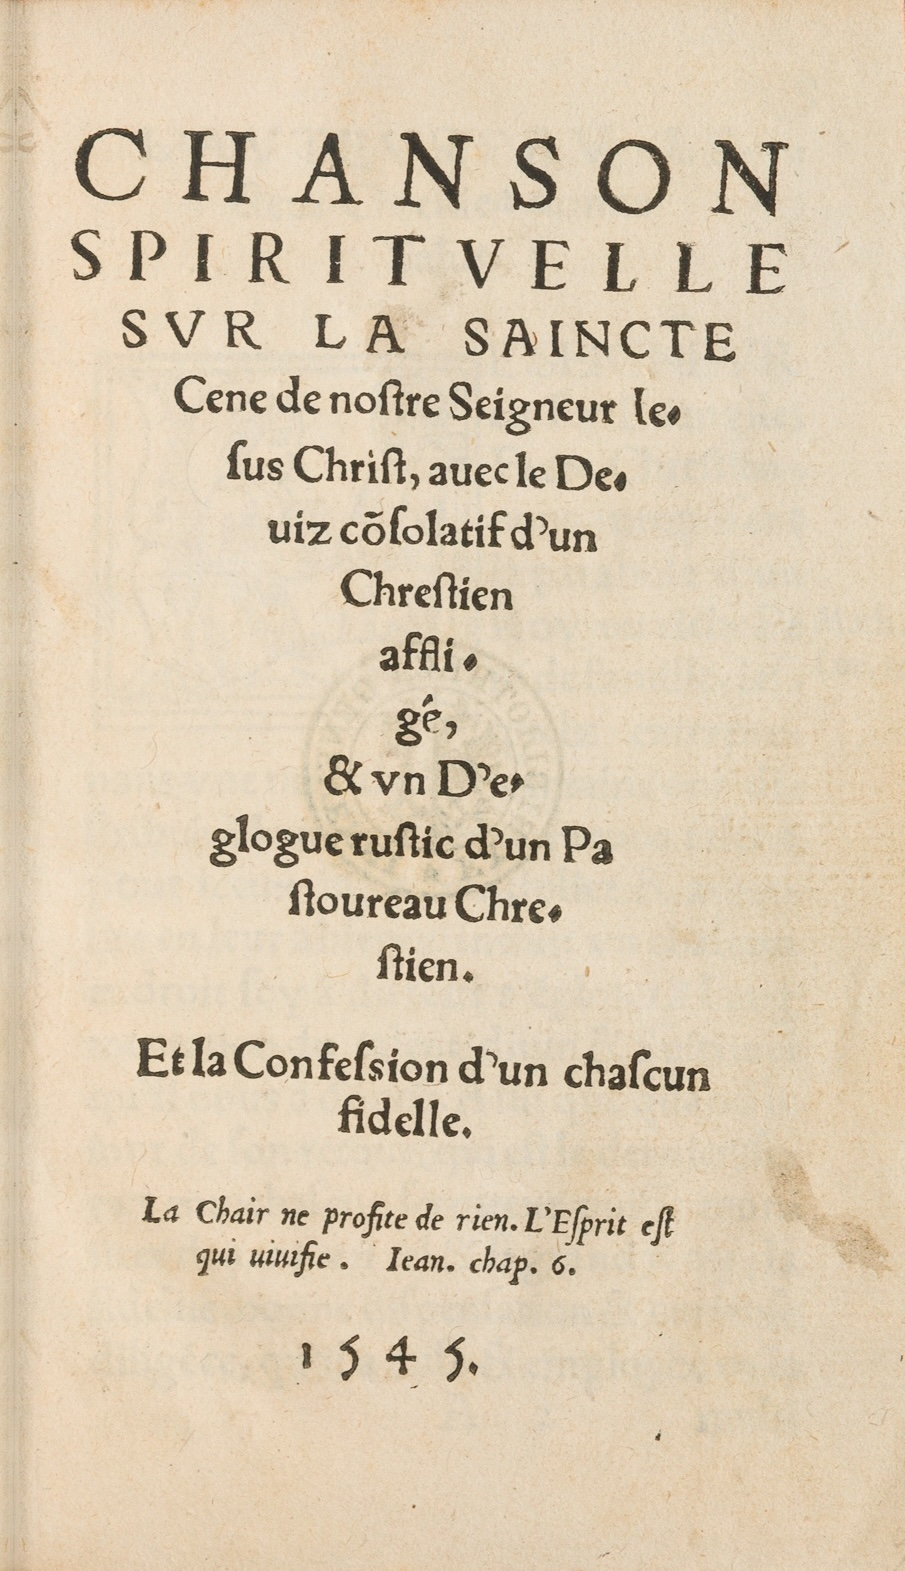
\includegraphics[width=.87\linewidth,height=6cm,keepaspectratio=false]{images/chanson-1545-29432242-original.jpeg}
        \caption{}
    \end{subfigure}
    \vspace{0.2cm}
    \hspace{0.2cm}%
    \begin{subfigure}[t]{.31\linewidth}
        \centering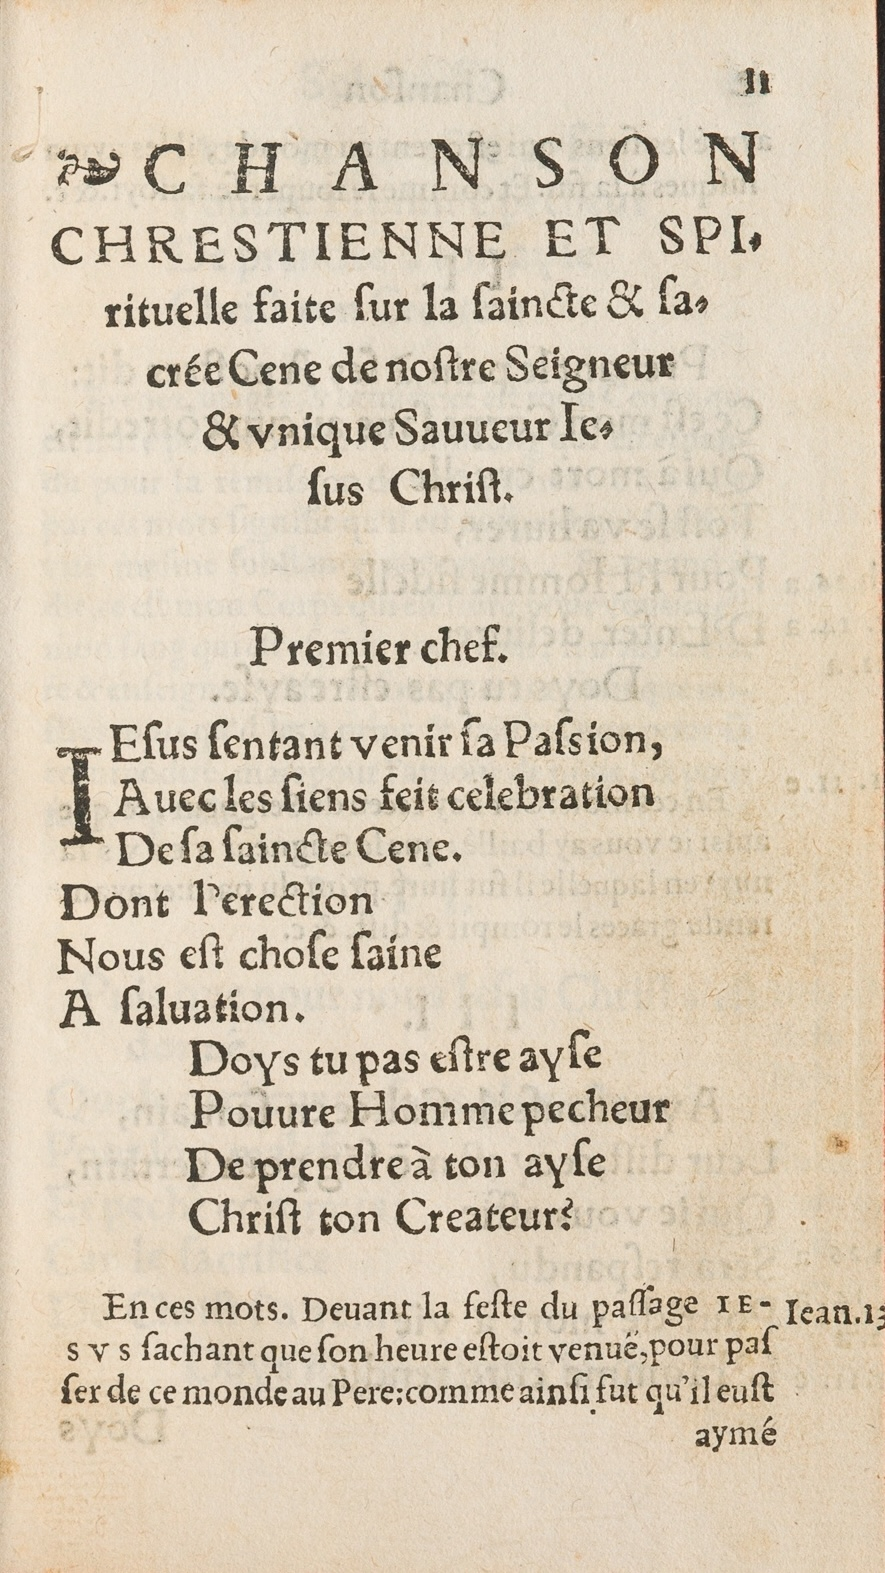
\includegraphics[width=.87\linewidth,height=6cm,keepaspectratio=false]{images/chanson-29432252-original.jpeg}
        \caption{}
    \end{subfigure}
    \vspace{0.2cm}
    \hspace{0.2cm}%
    \begin{subfigure}[t]{.31\linewidth}
        \centering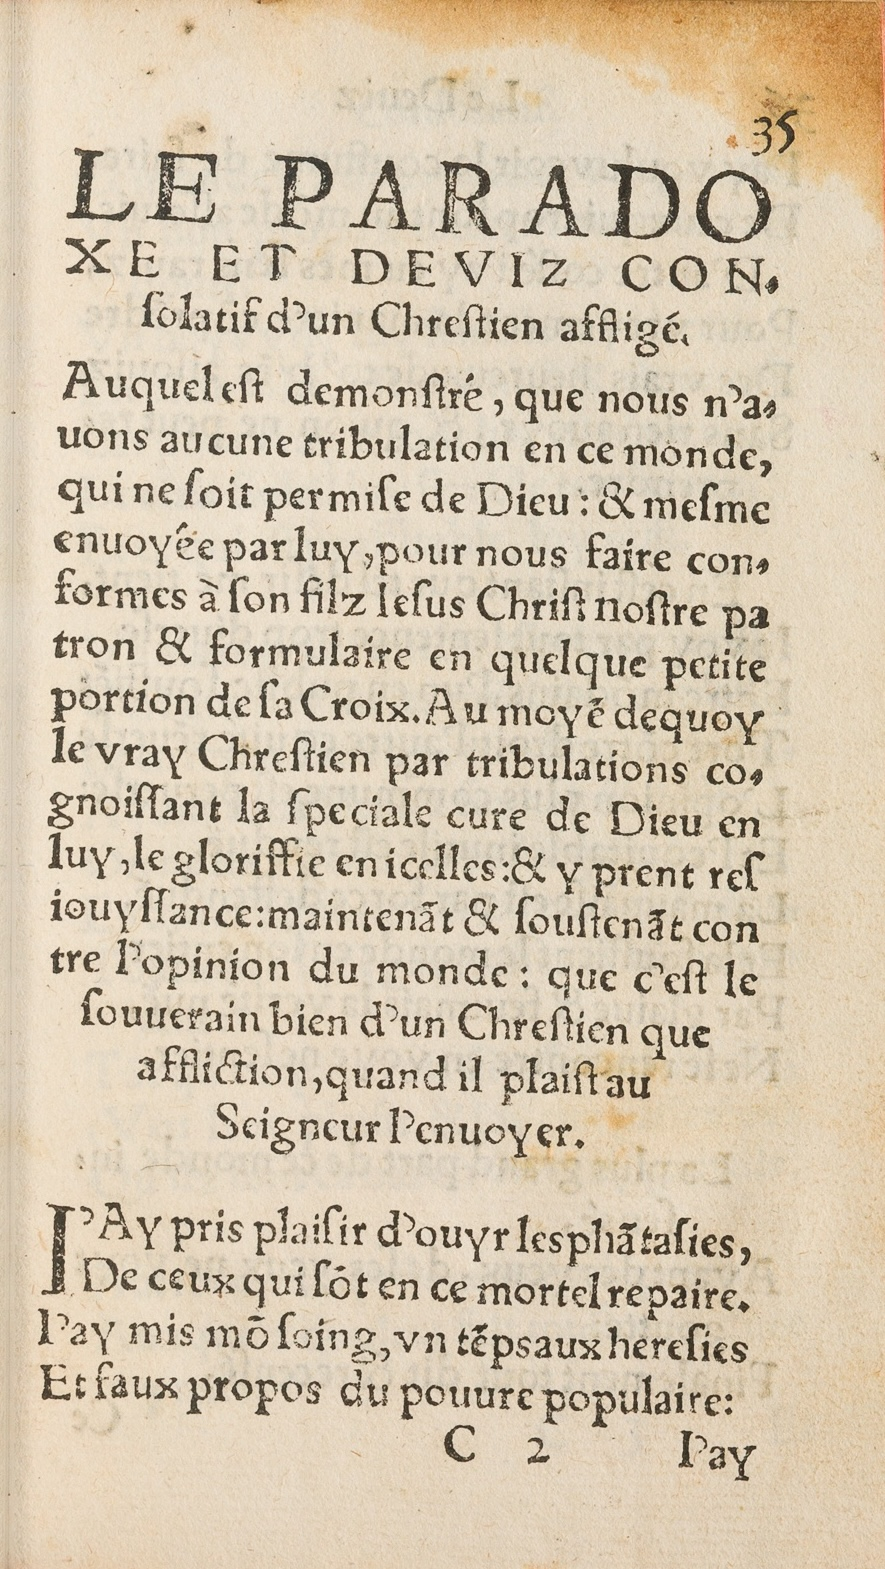
\includegraphics[width=.87\linewidth,height=6cm,keepaspectratio=false]{images/paradoxe-29432276-original.jpeg}
        \caption{}
    \end{subfigure}
    \vspace{-0.4cm}
  \caption{\textbf{(a)} La page de titre du recueil ; \textbf{(b)} la première page de la \textit{Chanson chrestienne et spirituelle} ; \textbf{(c)} la première page du \textit{Paradoxe}. Source des trois images : \textit{Chanson spirituelle sur la saincte Cene}. [s.l.] : [s.n.], 1545. (\href{https://doi.org/10.3931/e-rara-120199}{\underline{e-rara}}).}
  \label{fig:images_chanson1545}
    \vspace{-0.4cm}
\end{figure*}

\subsection{Débat sur l'attribution du recueil}
\label{sec:debat-cs}
En ce qui concerne les deux poèmes centraux du recueil, \textit{Le Paradoxe} et la \textit{Complaincte}, ils sont publiés en 1558, avec quelques variantes, dans deux éditions parisiennes d'Estienne Denise. Pour chaque édition il existe un seul exemplaire conservé au Département des Manuscrits de la Bibliothèque nationale de France\footnote{Exemplaires conservés à Paris, BnF, Rothschild 2859 (\href{https://archivesetmanuscrits.bnf.fr/ark:/12148/cc37294k}{\underline{notice}}) ; USTC \href{https://www.ustc.ac.uk/editions/41579}{\underline{n° 41579}} et \href{https://www.ustc.ac.uk/editions/41577}{\underline{n° 41577}}.}. \textit{Le Paradoxe} est présenté sous le titre \textit{Le Riche en pauvreté} et comme «~composé par Clément Marot et trouvé parmi ses autres factures à Chambery~», tandis que la \textit{Complaincte} est présentée comme «~trouvée après sa mort à Chambery~». Ces indications figurent sur les pages de titre de 1558, mais elles sont absentes dans l'édition de 1545.

Si la plupart des chercheurs convergent sur l'attribution de la \textit{Complainte} à Clément Marot, le débat sur \textit{Le Paradoxe} / \textit{Le Riche en pauvreté} reste encore ouvert \cite{higman2023, defaux2014marot2, screech1994marot}.
Concernant les autres pièces du recueil de 1545, découvert par Francis Higman vers 1997, ce dernier avance l’hypothèse selon laquelle Matthieu Malingre serait l’auteur le plus probable de toutes les pièces du recueil, à l’exception de la \textit{Complainte} \cite{higman_piety_2016,higman2023}. Une vingtaine d'années plus tard, Julien Goeury affirme que cette hypothèse est difficile à remettre en cause, mais il paraît relancer lui aussi le nom d'Eustorg de Beaulieu comme possible auteur du recueil \cite{goeury2016muse}.
Fr.~Higman avait envisagé en premier l'attribution au poète et musicien Eustorg de Beaulieu, mais il l’avait écarté principalement pour des raisons biographiques : Malingre entretenait des liens plus étroits avec Marot et aurait pu posséder un manuscrit de la \textit{Complainte} rédigée par ce dernier, avant de l’intégrer à un recueil issu de sa propre plume. 
Un tel scénario permettrait également d’expliquer les différences observées entre la \textit{Complainte} et les autres textes du recueil de 1545, notamment en ce qui concerne l’engagement doctrinal réformé et la présence de références bibliques en marge des textes, caractéristiques des chansons spirituelles réformées et non des chansons de Marot.

Malgré les raisons avancées par Fr.~Higman, il nous paraît raisonnable de conserver Beaulieu comme hypothèse de travail, dans la mesure où Malingre et Beaulieu recourent tous deux au \textit{contrafactum}, à la réécriture spirituelle de chansons profanes, au sein d'un même espace poétique \cite{ferrer2012chanson, ullberg2005salvation, vignes_introduction_2022}. Par ailleurs, Marot constitue un modèle poétique commun à Malingre et à Beaulieu, et ce dernier semble également s’inspirer des recueils de Malingre \cite{baranova2019}. Ces éléments invitent à envisager l’existence de possibles porosités stylistiques entre leurs productions\footnote{Pour d’autres cas d’attribution contestée entre Malingre et Marot, concernant deux pièces manuscrites conservées dans le recueil Grenet, voir G. Berthon et E. Doudet (2020), \cite{berthon_doudet_recueil_2020}. Voir également S. Solfrini, « Des remplois en concurrence : les réécritures spirituelles des chansons de Clément Marot par Matthieu Malingre et Eustorg de Beaulieu », à paraître dans les actes du colloque \textit{Le remploi comme pratique de communication religieuse : Matérialités, transferts, intertextualités au temps des Réformes (v. 1520-v. 1600)}, 11-13 mars 2026, Université de Genève.}.

\subsection{Corpus d'étude}
Pour notre analyse stylométrique, nous avons décidé de ne prendre en compte que les textes en vers du recueil de 1545, mais de retirer également la \textit{Complaincte} de nos expériences, celle-ci étant déjà attribuée à Marot avec un certain degré de certitude.
Le choix d'exclure la prose est fait pour des raisons techniques, car le type de texte comme sa forme font partie des nombreux paramètres à considérer, dans la mesure où ils ont leur propre signal et peuvent donc brouiller celui de l'auteur.
Au final, les vers retenus pour nos expériences comptent environ $3~000$ mots et correspondent aux pièces suivantes : les parties en vers de la \textit{Chanson chrestienne et spirituelle} ; \textit{Le Paradoxe} / \textit{Le Riche en pauvreté} ; le huitain et les deux prières finales (cf. § \ref{sec:content-cs}).

\section{Méthode} \label{sec:method-training}

\subsection{Corpus d'entraînement}
Concernant le corpus de comparaison, nous avons travaillé sur environ $6~000$ mots par auteur :

\begin{itemize}
    \item Pour Malingre, une partie des chansons spirituelles contenues dans \textit{Plusieurs belles et bonnes chansons} ([Neuchâtel] : [Pierre de Vingle], 1533)\footnote{Exemplaire conservé à Genève, Bibliothèque de Genève, BGE Cth 2650 (1) / BGE Bd 1475 (1) (\href{https://swisscovery.slsp.ch/permalink/41SLSP_UGE/cao1fn/alma991031959519705501}{\underline{notice}}). %; GLN 15-16 n° 4822, USTC n° 9720.
    } et dans les \textit{Noelz nouveaulx} ([Neuchâtel] : [Pierre de Vingle], ca.~1533)\footnote{Exemplaire conservé à Zurich, Zentralbibliothek Zürich, Res 1332 (\href{https://swisscovery.slsp.ch/permalink/41SLSP_UGE/hou1g5/alma991050231369705501}{\underline{notice}}). %; GLN 15-16 n° 4500, USTC n° 9752.
    } ;
    \item Pour Marot, une partie des rondeaux et des chansons contenues dans l'\textit{Adolescence clémentine} (Lyon : Gryphius, 1538)\footnote{Exemplaire conservé à Paris, BnF, RES-YE-1461 (\href{https://catalogue.bnf.fr/ark:/12148/cb30888593j}{\underline{notice}}). %; USTC n° 11087.
    } ;
    \item Pour Beaulieu, une partie des chansons spirituelles contenues dans la \textit{Chrestienne resjouyssance} ([Genève] : [Jean Girard], 1546)\footnote{Exemplaire conservé à Vienne, ÖNB, 80.M.74 (\href{https://search.onb.ac.at/permalink/f/sb7jht/ONB_alma21282574320003338}{\underline{notice}}). %; GLN 15-16 n° 1450, USTC n° 29595.
    }.
\end{itemize}

\subsection{Préparation des données}
Pour préparer nos données (corpus d'étude et d'entraînement), nous avons transcrit les textes à l'aide de modèles d'ATR (\textit{Automatic Text Recognition}) et nous avons corrigé manuellement ces transcriptions, grâce à une instance d'eScriptorium \cite{unige_fondue, kiessling2019escriptorium,solfrini2024ocr}. Les textes sont ensuite convertis au format XML-TEI, puis normalisés orthographiquement (cf. § \ref{sec:etat-art})\footnote{Les principes de normalisation que nous avons adoptés feront l’objet d’un chapitre dans un manuel à paraître.}. Nous rappelons que cette dernière étape est fondamentale pour que l'analyse stylométrique soit faite sur le lexique sans tenir compte d'un vêtement graphique encore instable à cette époque.
Enfin, nous avons converti les textes au format TXT et nous avons retiré tous les noms propres pour éviter qu'ils soient pris en compte dans le calcul des fréquences lexicales.

\subsection{Paramétrage}

Nos expériences reposent sur un classifieur à vecteurs de support (SVM) tel qu'implémenté dans SuperStyl \cite{camps_cafiero_2024} (cf. § \ref{sec:etat-art}).
Le corpus d’entraînement est segmenté en échantillons de taille variable, allant de 500 à 2~000 tokens, chaque taille de bloc définissant une condition expérimentale distincte.
Pour chacune de ces configurations, plusieurs stratégies de correction du déséquilibre des classes sont évaluées, incluant le sur-échantillonnage, le sous-échantillonnage et la pénalisation du modèle, via la pondération des classes dans la fonction objectif de la SVM. La représentation stylistique des textes est également variée, en considérant successivement et combinatoirement des \textit{features} différentes: des trigrammes de caractères, des affixes morphologiques et des mots-outils \cite{kestemont2014, sapkota2015}.
Les vecteurs de traits sont normalisés par norme L2 et les performances sont estimées au moyen d’une validation croisée à 10 plis ($k = 10$), assurant la robustesse des résultats pour l’ensemble des paramètres évalués.
% SS OLD: Au-delà des paramètres standards, maintenus constants — normalisation L2, stratégie combinant pondération des classes et sous-échantillonnage, et validation croisée de type \textit{k-fold} — nous avons testé plusieurs configurations, faisant varier la taille des échantillons ainsi que les \textit{features} utilisées (trigrammes de caractères, mots-outils, affixes, ou des combinaisons de ces éléments) \cite{kestemont2014, sapkota2015}.
% SG OLD: Le corpus d’entraînement est segmenté de manière systématique en blocs de taille variable, allant de 500 à 2000 tokens (SS: tokens ou mots? c'est words dans les scripts), avec un pas de 250 tokens (SS: 250? c'est 10 ou 150 dans mes scripts), chaque taille de bloc définissant une condition expérimentale distincte. Pour chacune de ces configurations, plusieurs stratégies de correction du déséquilibre des classes sont évaluées, incluant le sur-échantillonnage, le sous-échantillonnage et la pénalisation du modèle via la pondération des classes dans la fonction objectif de la SVM. La représentation stylistique des textes est également variée, en considérant successivement et combinatoirement des trigrammes de caractères, des distributions de mots vides et des affixes morphologiques. Les vecteurs de traits sont standardisés sous forme de cotes z (SS: je ne comprend pas ici), puis normalisés par norme L2. Différents noyaux SVM sont évalués, à savoir les noyaux linéaire, à fonction de base radiale (RBF) et sigmoïde, afin d’analyser l’impact de la fonction de décision sur les performances de classification (SS: je ne comprend pas ici). Les performances sont estimées au moyen d’une validation croisée à 10 plis ($k = 10$), assurant la robustesse des résultats pour l’ensemble des paramètres évalués.

\begin{table}[htp]
    \centering
    \begin{tabular}{l|cccc}
        \toprule
               & Précision & Rappel & F1-mesure & Support \\
        \midrule
        Beaulieu      & 1.00 & 0.83 & 0.91 & 6\\
        Malingre      & 1.00 & 1.00 & 1.00 & 5\\
        Marot         & 0.86 & 1.00 & 0.92 & 6\\
        \midrule
        Exactitude &  &  & 0.94 & 17\\
        Moyenne macro & 0.95 & 0.94 & 0.94 & 17\\
        Moyenne micro & 0.95 & 0.94 & 0.94 & 17\\
        \bottomrule
    \end{tabular}
    \caption{Performance du meilleur modèle de classification (trigrammes de caractères, échantillons de $1~000$ tokens, sous-échantillonnage et pénalisation du modèle).}
    \label{tab:results}
\end{table}

L'utilisation des trigrammes de caractères, d'échantillons de $1~000$ tokens, d'un sous-échantillonnage et d'une pénalisation du modèle apparaît comme la configuration la plus robuste (tab. \ref{tab:results}). Elle combine de très bonnes performances (exactitude = 0,94) avec un nombre suffisant de segments (17 au total, répartis de manière équilibrée entre les trois auteurs).

\section{Résultats} \label{sec:results}

\begin{figure}[h]
  \centering
  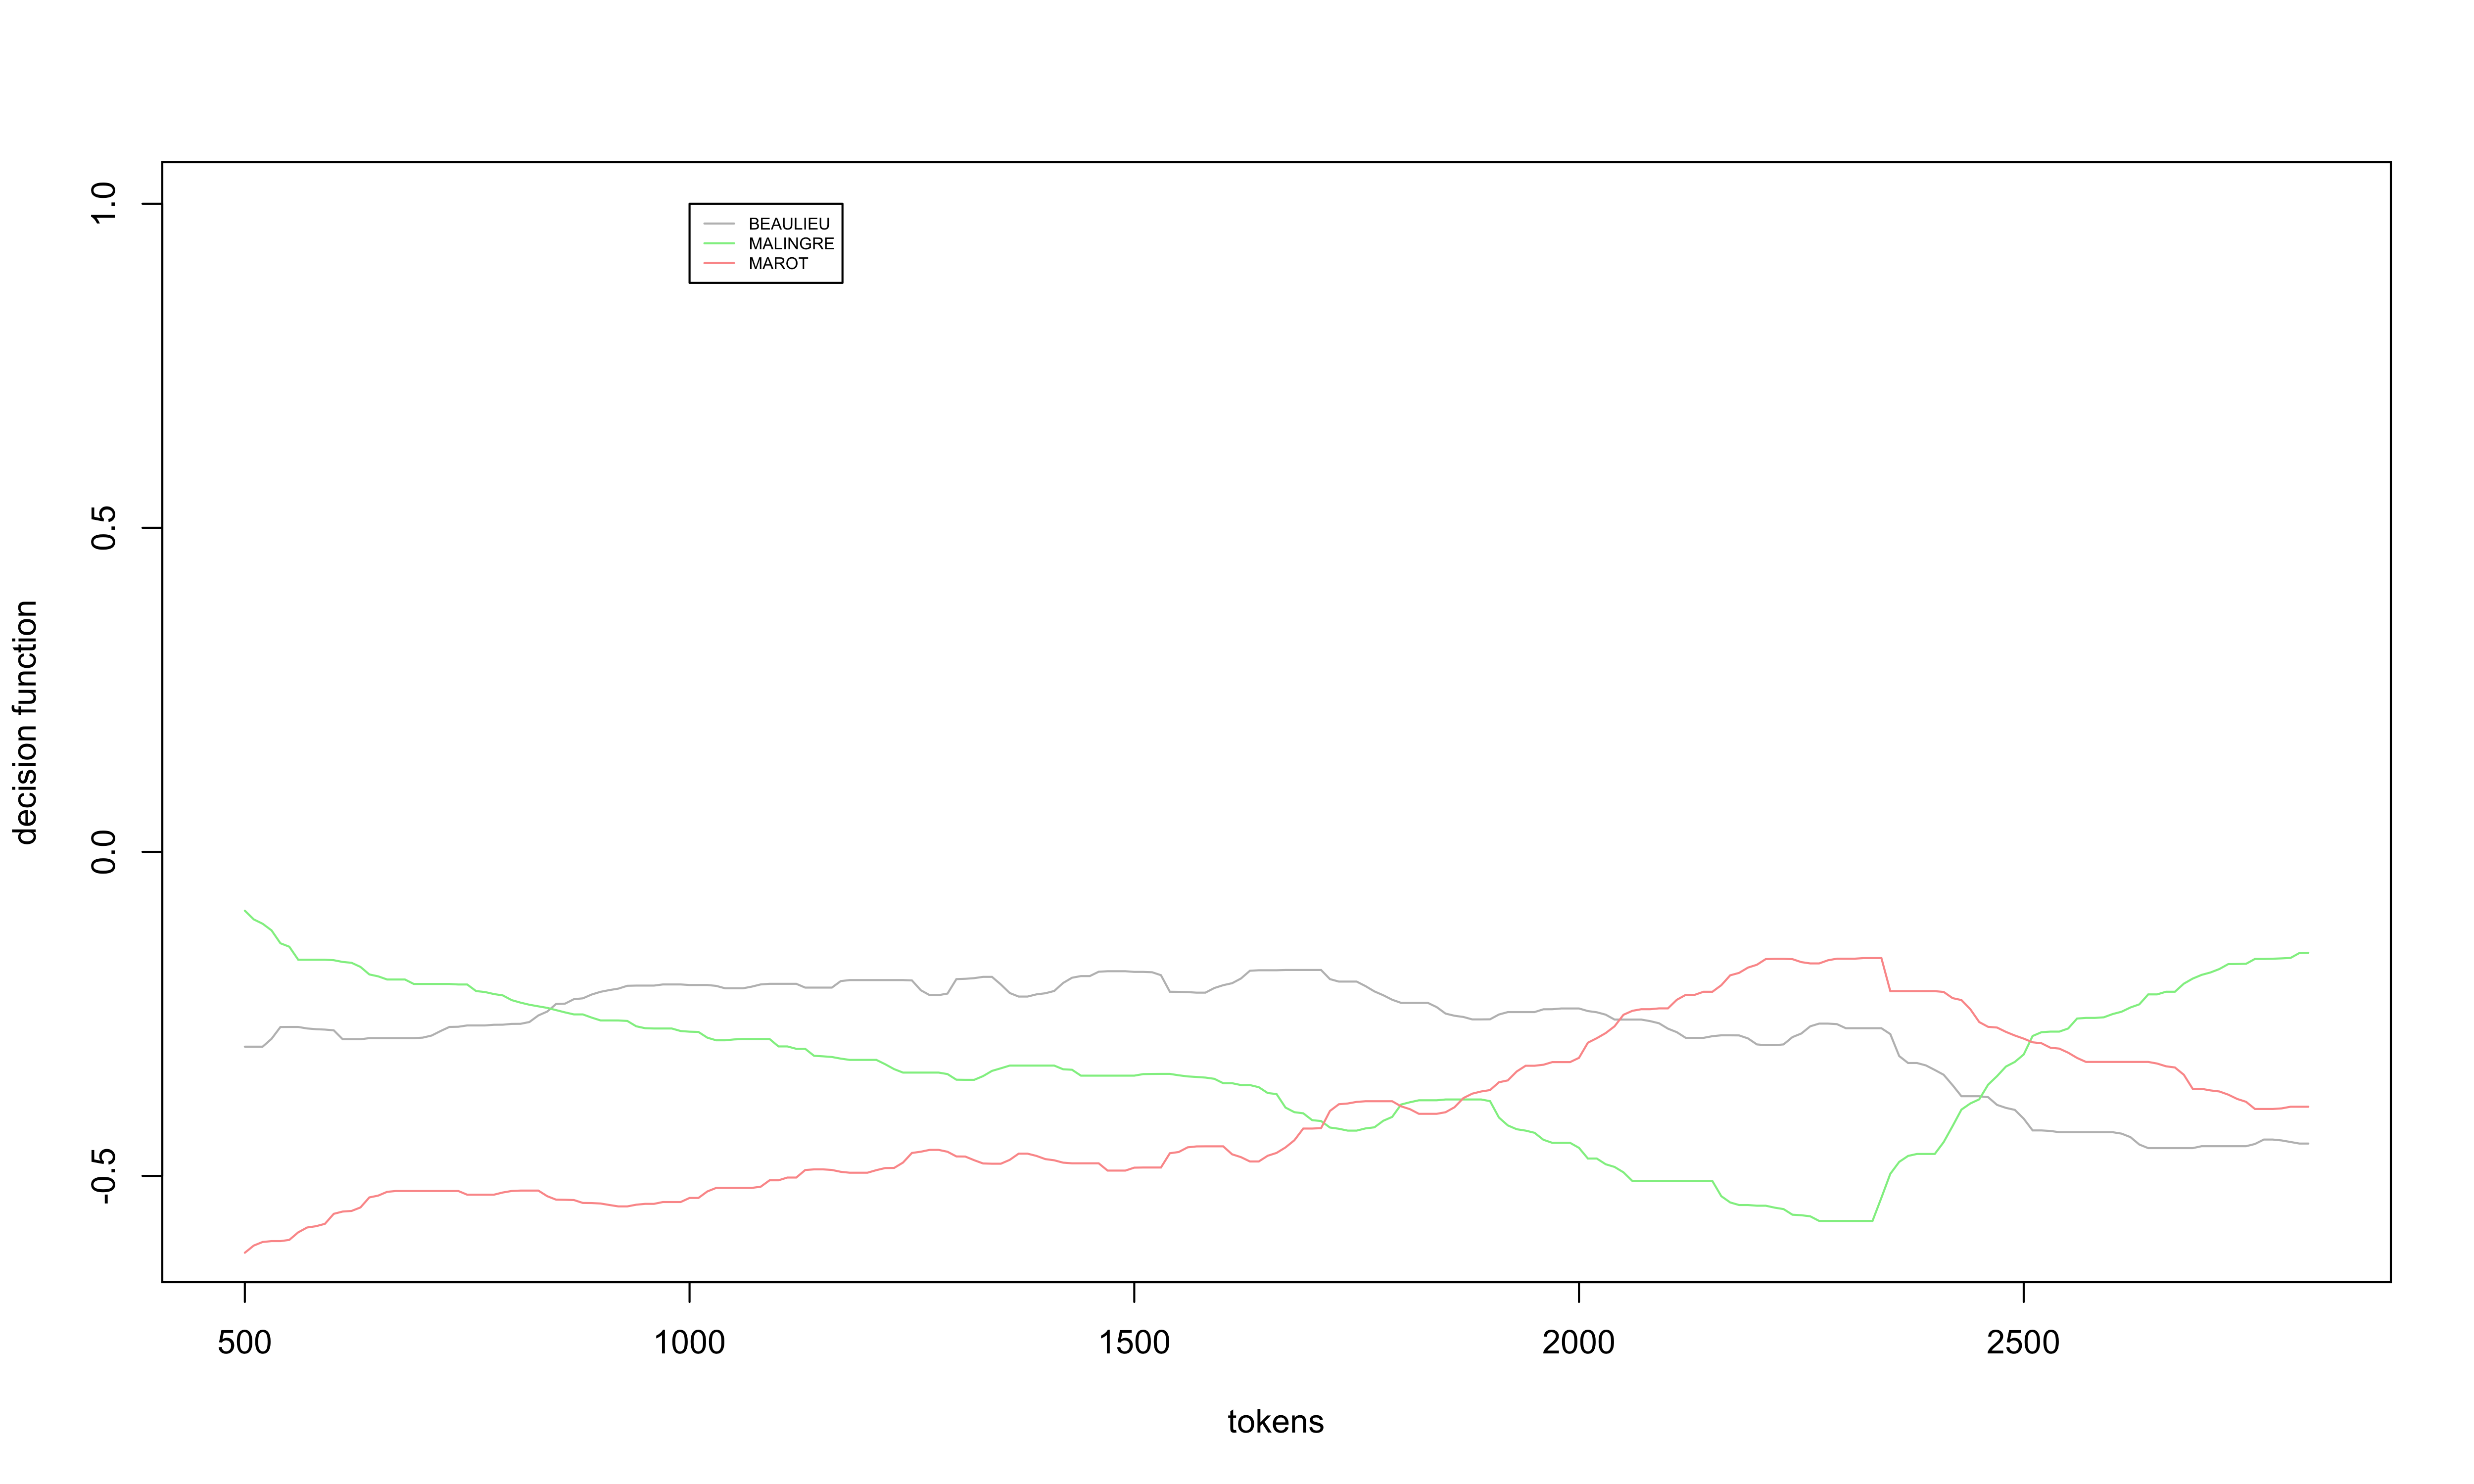
\includegraphics[width=1\linewidth]{images/rolling_1000_chars3.png}
  \caption{Analyse roulante du corpus d'étude, avec la meilleure configuration de la SVM et un pas de 10 tokens. Les pièces sélectionnées du recueil sont concaténées les unes à la suite des autres.}
  \label{fig:rolling}
\end{figure}
% SS : voir la 2eme expertise "Serait-il possible d'ajouter dans la figure 3, en abscisse, une indication des différentes parties de l'œuvre concernée (pour faire écho à la discussion de la section 5) ?"

Afin d’examiner l’évolution des attributions au fil des pièces retenues, nous avons recours à une analyse dite «~roulante~» (\textit{rolling analysis}) \cite{eder2015rolling}. Le texte est découpé en segments de longueur fixe ($1~000$ tokens), se chevauchant selon un pas de 10 tokens, puis chaque segment est soumis au classifieur préalablement entraîné. Les scores de décision associés à chaque auteur sont ensuite reportés à la position correspondante dans le texte, ce qui permet de visualiser la dynamique attributionnelle tout au long de l’ouvrage. En effet, il se peut que certains pièces du recueil soient d'un auteur, et d'autres textes d'un autre auteur.

% tot 3.230 
Les parties en vers de la \textit{Chanson chrestienne et spirituelle} (ca.~700 mots), \textit{Le Paradoxe / Le Riche en pauvreté} (ca.~2~000 mots), le huitain (ca.~60 mots) et les deux prières finales (ca.~130 et 240 mots) sont rassemblés à la suite les uns des autres, la SVM opérant sur des échantillons de 1~000 tokens. Si l'on constate l'absence de signal clairement positif (i.e. $>$ 0, fig.~\ref{fig:rolling}), on observe tout de même des changements assez nets dans les prédictions, avec le signal de Malingre qui ressort pour la \textit{Chanson chrestienne} et les trois derniers poèmes (huitain et prières). Pour la partie centrale, celle du \textit{Paradoxe}, c'est en revanche le signal de Beaulieu qui se dégage pour les deux premiers tiers, légèrement dépassé par celui de Marot pour la partie finale.

\section{Discussion} \label{sec:conclusions}

Ces résultats ne permettent pas, à ce stade, d'attribuer les différentes pièces analysées du recueil à l'un ou l'autre auteur. On remarque toutefois que les parties versifiées de la \textit{Chanson chrestienne} ainsi que les trois coutres pièces conclusives font ressortir le signal stylométrique de Malingre de manière assez nette, et ce malgré leur faible volume ($<$ 1~000 tokens) qui les contraint à être mélangées avec des extraits du \textit{Paradoxe} lors de l'analyse roulante. 
% Ce signal atteint son intensité maximale là où la proportion de données issues de cette dernière pièce est la plus réduite.
Pour ce qui est du \textit{Paradoxe}, l'analyse est plus complexe: le signal de Beaulieu domine les deux premiers tiers, tandis que celui de Marot le supplante dans le troisième tiers. Plutôt que d'y voir un changement de plume, il est possible d'interpréter ce croisement comme la mobilisation d'un hypotexte marotien dont le rôle dans la constitution du modèle poétique de Beaulieu est bien attesté (cf. § \ref{sec:debat-cs}).

% SS OLD : Afin de déterminer si l’attribution à Beaulieu reflète effectivement un signal d’auteur, il serait nécessaire d’introduire un quatrième auteur de contrôle dans l’analyse. Si le signal associé à Beaulieu se maintenait à un niveau élevé, l’hypothèse de son attribution en serait renforcée ; dans le cas contraire, une baisse du signal indiquerait plutôt un effet de compétition entre profils stylistiques.
% SS : quoi faire de ce paragraphe ? voir les expertises

Ces expériences ayant été menées sur un corpus de taille réduite (environ $6~000$ mots par auteur), ces résultats préliminaires gagneraient à être consolidés par un élargissement des données d’entraînement. Une telle extension pose toutefois des défis, notamment en matière de prétraitement des données. Des solutions comme la transcription automatique peuvent être utiles ; mais, pour les textes du \textsc{xvi}\textsuperscript{e} siècle, l’obtention d’une normalisation orthographique de bonne qualité demeure encore particulièrement chronophage. En outre, nos expériences ont été réalisées sur un corpus exclusivement composé de textes en vers, alors que le recueil étudié contient également des passages en prose (les commentaires de la \textit{Chanson chrestienne} et \textit{La Confession du fidelle Chrestien}). L’étude de leur paternité impliquerait un changement d’approche, dans la mesure où les trois auteurs considérés ont très rarement, voire jamais, écrit en prose. Enfin, d’autres méthodes d’analyse stylométrique pourraient également être envisagées pour l’étude des pièces en vers.

Pour conclure, dans le contexte francophone du \textsc{xvi}\textsuperscript{e} siècle, si l’on observe l’émergence d’une conscience d’auteur et l’importance d’afficher son nom, l’anonymat des ouvrages – complet ou partiel (noms de plume, anagrammes, acrostiches, etc.) – demeure très courant, notamment dans la littérature polémique \cite{dauvois_acrostiches_2008,bodenmann_lauteur_2009,walsby_voix_2009,walsby_lauteur_2012}. De surcroît, dans ce type de production, les pratiques d’écriture collaborative sont également fréquentes, et certains textes sont rédigés à plusieurs mains \cite{szczech2021groupe,desrosiers_atelier_2014,reach-ngo_du_2015}. À cela s’ajoute l’absence fréquente du nom de l’imprimeur et du lieu de publication. Dans ce cadre complexe, la stylométrie apparaît comme un outil encore peu mobilisé pour l’attribution des écrits de la Renaissance, mais dont le potentiel pourrait être davantage exploré.

\section*{Financement}

Les recherches ont été menées dans le cadre du projet \href{https://www.unige.ch/setaf/}{\underline{SETAF}} (FNS \href{https://data.snf.ch/grants/grant/205056}{\underline{n° 205056}}).

\section*{Remerciements}
Nous remercions nos relecteur·trice·s anonymes et Daniela Solfaroli Camillocci pour leur relecture et leurs suggestions.

% Imprime la bibliographie à la fin. Gardez cette ligne après le texte principal de votre article et avant une annexe.
\printbibliography

% Vous pouvez inclure une annexe en utilisant la commande suivante
\appendix

%\section{Première section de l'annexe} \label{appdx:first}

%Des annexes facultatives peuvent être ajoutées après la section des références. 

\end{document}